\documentclass[9pt,shortpaper,twoside,web]{ieeecolor}
\usepackage{generic}
\usepackage{cite}
\usepackage{amsmath,amssymb,amsfonts}
\usepackage{algorithmic}
\usepackage{graphicx}
\usepackage{textcomp}
\usepackage[utf8]{inputenc}
\usepackage[T1]{fontenc}

\def\BibTeX{{\rm B\kern-.05em{\sc i\kern-.025em b}\kern-.08em
    T\kern-.1667em\lower.7ex\hbox{E}\kern-.125emX}}
\markboth{\journalname, Research and documentation project}
{Author \MakeLowercase{\textit{et al.}}: O scurtă prezentare a metodelor de detectare a emoţiilor din semnalul vocal (Mai 2018) }

\begin{document}
\title{
O scurtă prezentare a \\
metodelor de detectare a emoţiilor din semnalul vocal  \\ 
(Mai 2018)}
\author{Iordache-Stoicescu Laurențiu-Iulian}

\maketitle


\begin{abstract}
Aplicațiile de clasificare a emoțiilor sunt folosite pentru a îmbunătăți percepția mașinii asupra semanticii mesajului transmis de utilizator. În aplicațiile de clasificare a emoțiilor pe baza semnalului audio, caracteristicile utilizate cu precădere sunt cele ce țin de statistica frecvenței fundamentale, conturul energiei, durata porțiunilor de liniște și calitatea vocii. Performanța acestor sisteme scade atunci când sunt prezente mai multe emoții în semnalul audio. În acest articol s-a realizat o prezentare a caracteristicilor prezente în semnalul vocal pe baza cărora se pot determina emoțiile, a factorilor care influențează aceste caracteristici precum și o analiză a câtorva metode de deducere a unor emoții. 
\end{abstract}

\begin{IEEEkeywords}
PAD - Pleasure-Arousal-Dominance
HMM – Hidden Markov Model
SVM – Support vector machine
LPC - Linear Predictor Coefficients
MFCC - Mel-frequency Cepstrum Coefficients
LFPC -  Log-frequency power coefficients
\end{IEEEkeywords}


\section{Introducere}
\label{sec:introduction}
Semnalul vocal reprezintă cea mai rapidă metodă naturală de comunicare între oameni. Acest fapt a determinat apariția multor interfețe de comunicare om-mașină pentru a eficientiza metoda de interacțiune dintre om și mașină. În ciuda tuturor progreselor realizate în recunoașterea vorbirii, este încă grea realizarea unei interacțiuni naturale între om și mașină deoarece mașina nu pricepe emoțiile vorbitorului. Datorită acestei necesități a apărut ramura de recunoaștere a emoțiilor din vorbire, aceasta se ocupă cu analizarea stării emoționale a vorbitorului pentru a oferi diverse semantici mesajului transmis de către acesta.


\subsection{Necesitate}
Recunoașterea emoțiilor din vorbire este folositoare în aplicații care necesită o interacțiune naturală între utilizator și mașină cu ar fi filme web și aplicații de învățare pentru care sunt necesare ca răspuns emoțiile utilizatorului. De asemenea, recunoașterea emoțiilor mai sunt importante și în aplicații de bord ale autovehiculelor în care informația legată de starea mentală a șoferului poate fi utilizată în favoare siguranței acestuia. O altă aplicație în care se poate utiliza recunoașterea emoțiilor o reprezintă sistemele de traducere automată în care simpla stare a utilizatorului poate varia înțelesul traducerii.


\subsection{Generalități}
Sarcina de detecție a emoțiilor este o sarcină complicat de realizat. Nu este clar ce caracteristici ale vorbirii sunt importante pentru distingerea emoțiilor. Pe lângă această incertitudine se mai adaugă și variabilitatea semnalului introdusă de diversitatea propozițiilor, vorbitorilor, ciclurilor de vorbire și a vitezelor de vorbire. Această sarcină mai este îngreunată și de faptul că de cele mai multe ori nu este prezentă o singură emoție la un vorbitor, acestea există cumulativ în enunțurile rostite deoarece. Încă un motiv este acela că manifestarea emoțiilor variază de la de la un vorbitor la altul și pe baza culturii și a mediului acestuia. 

Emoțiile nu au o definiție teoretică ce este acceptată de toată lumea. Este foarte întâlnit ca acestea să fie caracterizate în două tipuri:


\subsubsection{De activare}
Activarea se referă la cantitatea de energie necesară pentru a exprima o anumită emoție.

Anumite emoții cum ar fi bucuria, furia și frica provoacă o creștere a pulsului, a tensiunii, schimbări ale ritmului respirației, presiune sub-glotală mărită, uscare a gurii și ocazional tremurări musculare. Toate aceste modificări fiziologice provoacă schimbări în caracteristicile acustice ale mesajului transmis. Mesajul este enunțat rapid cu sonor ridicat și o frecvență audio ridicată.

Alte emoții cum ar fi tristețea induc efecte inverse față de cele anterior menționate și anume scăderea pulsului și a tensiunii, creșterea gradului de umiditate a gurii. Aceste emoții determină un mesaj audio ce este rostit la intensitate scăzută, cu mai puține frecvențe înalte.


\subsubsection{De valență} 
De valență: Emoțiile nu pot fi caracterizate doar având în vedere nivelul de energie necesar. De exemplu, bucuria și furia sunt ambele emoții cu un nivel mare de energie dar afectează diferit. Această diferență este caracterizată de dimensiunea valenței. Din nefericire nu se știe precis cum această valență afectează caracteristicile acustice pentru alte emoții. De aceea, clasificarea între emoțiile de excitare înaltă și cele de excitare joasă se poate realiza cu precizie ridicată iar clasificarea dintre diferite alte emoții este încă greu de realizat.

O altă chestiune importantă în recunoașterea emoțiilor constă în alegerea unui set definit de emoții. Lingviștii au definit un set de aproximativ 300 de emoții pe care le întâlnim pe parcursul vieții. Acest pachet de emoții este însă prea mare pentru a putea fi utilizat momentan, de aceea se recurge la utilizarea unui set restrâns de emoții de bază. O idee foarte interesantă este aceea că emoțiile pot fi descompuse în aceste emoții de bază precum culorile pot fi descompuse în culori primare. Emoțiile primare sunt definite de psihologul Paul Ekman ca fiind: tristețe, agonie, furie, surprindere, frică, dezgust și bucurie \cite{b6}.


\subsection{Baza de Date}
O chestiune importantă de luat în calcul în evaluarea unui sistem de recunoaștere a emoțiilor din vorbire este gradul de naturalețe al bazei de date utilizată în evaluarea performanțelor. Se pot trage concluzii incorecte despre sistem dacă datele utilizate nu sunt de calitate.

Din păcate, majoritatea bazelor de date cu date audio ce conțin înregistrări preluate de la vorbitori cu anumite emoții nu sunt disponibile public. Acest fapt determină o îngreunare a procesului de evoluție în această ramură. Cercetătorii nu sunt capabili sa se coordoneze din punctul de vedere al greșelilor și le repetă pentru baze de date diferite.


\subsection{Fapt}
În carlinga avioanelor s-a descoperit  că sistemele de recunoaștere a vorbirii antrenate cu mesaje de la un subiect aflat sub stres au performanțe mult mai bune decât sistemele antrenate cu mesaje de la subiecți aflați în stare normală.


\section{Emoțiile}
Cuvântul emoție este adese considerat ca fiind o stare afectivă a minții. În conversațiile umane normale, oamenii sunt capabili să identifice emoțiile altora pe baza vocii, a posturii, a gesturilor și a expresiei faciale. Emoțiile sunt adesea neglijate în interacțiunea dintre om și mașină. Pentru a putea detecția emoțiilor trebuie determinate trei aspecte:

\begin{itemize}
\item Ce reprezintă o stare afectivă?

\item Ce semnale din comunicația verbală exprimă informația despre starea afectiva?

\item Cum ar trebui combinate diversele caracteristici pentru a optimiza percepția emoțiile de către mașină?
\end{itemize}


În literatură, emoțiile enumerate de Ekman (furie, dezgust, frică, fericire, tristețe și surprindere) sunt folosite cu precădere. Au fost propuse mai multe modele de ilustrare a relațiilor dintre valențe, excitare și emoții. Figura 1 prezintă modelul PAD al stărilor emoționale o analiză a emoțiilor propuse de alt psiholog, Russell \cite{b5}.

\begin{figure}[htb]
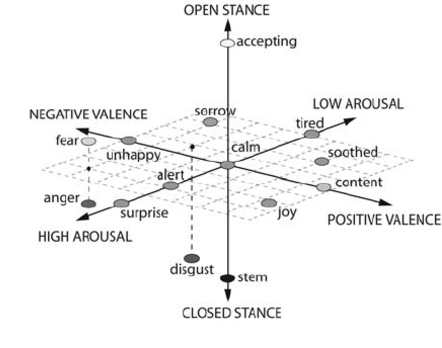
\includegraphics[width=0.9\columnwidth]{res/fig/pad-model-3D}
\caption{Modelul PAD 3D de clasificare a emoțiilor \cite{b7}}
\label{fig1}
\end{figure}

Din acest model se disting următoarele:

\begin{itemize}
\item Excitarea(Arousal) - emoțiile sunt caracterizate pe baza nivelului lor de excitare. 

\item Valență - emoțiile sunt caracterizate în funcție de cât sunt de pozitive sau de negative. Emoțiile pozitive sporesc atenția și alte funcții cognitive ale unei persoane
\end{itemize}


\section{Caracteristici utilizate pentru recunoașterea emoțiilor}
Pentru realizarea unui sistem de recunoaștere a emoțiilor din vorbirea unui subiect este necesară identificarea caracteristicilor ce caracterizează diversele emoții. O alegerea caracteristicilor va influența performanțele sistemului.

Pentru o analiză eficientă a caracteristicilor trebuie să se țină seama de regiunea de analiză utilizată pentru extragerea caracteristicilor, să se aleagă caracteristica potrivită pentru identificarea emoției, să se ia în calcul efectele proceselor uzuale de procesare a semnalului vocal cum ar fi filtrarea și eliminarea zonelor de liniște dar și de asemenea să se ia în calcul faptul că trăsăturile acustice s-ar putea să nu fie suficiente pentru modelarea emoțiilor și că ar putea să se folosească și alte tipuri de caracteristici cum ar fi informația discursului sau trăsăturile faciale. În continuare vor fi detaliate aceste aspecte.


\subsection{Caracteristici locale și caracteristici globale}
Primul aspect se referă la selectarea regiunii de analiză folosită pentru extragerea caracteristicilor. Aici există două abordări. Divizarea semnalului în cadre de durată scurtă pentru care se calculează vectorul caracteristic sau extragerea de mărimi statistice globale pentru întreaga propoziție. 

Deoarece semnalul vocal este nestaționar, se practică divizarea acestuia în ferestre mici de 20 până la 40 de ms. O caracteristică importantă a semnalului vocal, care facilitează analiza acestuia este că acesta este aproximativ staționar pe perioade scurte de timp. Din fiecare astfel de fereastră sunt extrase caracteristici prozodice cum ar fi frecvența fundamentală și energia și denumite caracteristici locale. 

Pe de altă parte, caracteristicile globale reprezintă statistici ale tuturor caracteristicilor locale extrase din mesaj. Majoritatea cercetătorilor au agreat faptul că aceste caracteristici globale sunt superioare caracteristicilor locale din punct de vedere al preciziei și a timpului de clasificare. Caracteristicile globale mai au încă un avantaj față de cele locale și anume acela că sunt mult mai puține la număr, ceea ce facilitează o execuție mult mai rapidă a unor algoritmi cum ar fi cel de ”validare în cruce”. Algoritmul de validare în cruce reprezintă o tehnică de evaluare a modelelor predictive petiționând mostra originală într-un set de antrenare pentru antrenarea modelului și un set de evaluare \cite{b2}. Utilizarea acestora este eficientă doar în cazul distingerii emoțiilor de excitație înaltă (ex. furia, frica și bucuria) de cele de excitare joasă(ex. tristețea). Caracteristicile globale nu reușesc să realizeze o clasificare precisă a emoțiilor cu excitare similară de exemplu identificarea furiei față de bucurie. De asemenea, mai prezintă și dezavantajul că informația temporală prezentă în mesaj este pierdută. Și încă un dezavantaj îl reprezintă chiar faptul că sunt într-un număr mai mic decât caracteristicile locale deoarece s-ar putea să nu se poată antrena modele de tipul HMM sau SVM.

O altă abordare pentru extragerea de caracteristici o reprezintă segmentarea semnalului pe durate scurte pentru analiza fonemelor. Această abordare se bazează pe faptul că forma spectrului fonemelor variază în funcție de emoții. Această afirmație este valabilă doar pentru vocale.


\subsection{Clasificarea caracteristicilor}
Un aspect important în recunoașterea emoțiilor îl reprezintă extragerea caracteristicilor semnalului vocal care caracterizează eficient emoția din mesaj dar în același timp este independentă de vorbitor sau de conținutul lexical.

Caracteristicile vorbirii pot fi grupate în următoarele categorii: Caracteristici continue, caracteristici calitative, caracteristici spectrale și caracteristici bazate pe operatorul TEO. În figura 1 se pot observa exemple de caracteristici aparținând fiecărei categorii.

\begin{figure}[htb]
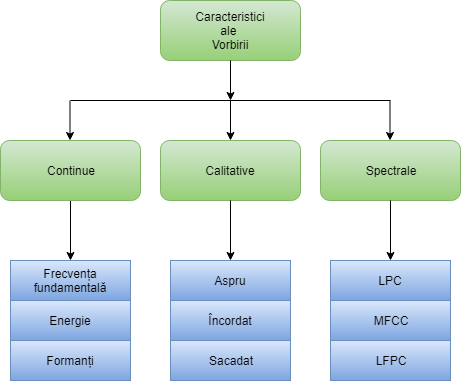
\includegraphics[width=0.85\columnwidth]{res/fig/clasificare-caracteristicilor}
\caption{Categorii de caracteristici ale semnalelor vocale}
\label{fig2}
\end{figure}

\subsubsection{Caracteristici de vorbire continue}
Caracteristicile prozodice continue cum ar fi frecvența fundamentală și energia exprimă o mare parte din sentimentele existente într-un mesaj. S-a observat că starea de excitare a subiectului influențează distribuția spectrală a energiei precum și frecvența și durata pauzelor din vorbire. Conform studiilor, aceste caracteristici acustice pot fi grupate în \cite{b1}:

\begin{itemize}
\item Caracteristici asociate frecvenței fundamentale;

\item Caracteristici bazate pe formanți

\item Caracteristici asociate energiei semnalului vocal

\item Caracteristici ale articulării
\end{itemize}


\subsubsection{Caracteristici de calitate a vocii}
Calitatea vocii este strâns legată de tipurile de emoții, aceasta este descrisă de emoții care direcționează puternic subiecții către un șir de acțiuni. Acestea sunt opuse emoțiilor fundamentale care influențează pozitiv sau negativ acțiunile și gândurile unei persoane. O gamă largă de variabile fonetice contribuie la impresia subiectivă de calitate a vocii. Corelațiile acustice sunt grupate în următoarele categorii \cite{b1}:

\begin{itemize}
\item Nivelul vocii, amplitudinea semnalului, energia și durata s-au dovedit a fi metrici bune pentru nivelul vocii.

\item Frecvența fundamentală a vocii

\item Fraze, foneme, cuvinte

\item Structurile temporale
\end{itemize}


\subsubsection{Caracteristici bazate pe spectru}
Acestea sunt adesea reprezentări ale semnalului pe perioade scurte de timp. Emoțiile dintr-un mesaj influențează distribuția spectrală de energie a mesajului. De exemplu, mesajele care sunt rostite când subiectul este fericit au un nivel ridicat al energiei pentru frecvențele înalte pe când cele rostite de subiecți care sunt triști emoțional au nivele scăzute ale energiei pentru aceleași frecvențe. 
Pentru o mai bună exploatare a gamei de frecvențe, spectrul este trecut printr-o serie de filtre trece-bandă. Caracteristicile spectrale sunt extrase pe baza rezultatelor obținute de la fiecare filtru. Deoarece percepția umană a frecvenței fundamentale nu este modelată liniar, filtrele trece-bandă sunt distribuite uniform cu privire la o  metodă neliniară potrivită cum ar fi scala frecvențelor Mel. 


\subsection{Procesarea vorbirii}
Înaintea extragerii caracteristicilor este necesară o preprocesare a semnalului audio. De exemplu, datorită diferențelor din mediul de înregistrare este necesară o normalizare a energiei pentru toate mesajele. Alt exemplu îl reprezintă netezirea contururilor extrase, pentru aceasta se folosește metoda suprapunerii cadrelor. Pentru eliminarea ondulațiilor din spectrul de frecvențe sunt utilizate ferestre de tip Hamming.

Deoarece intervalele de liniște pot oferi informații importante asupra stării emoționale, acestea sunt păstrate intacte, față de procesele normale de analiză a vorbirii.

Odată extrase caracteristicile se poate să fie necesară o postprocesare înainte de a antrena clasificatorul. De exemplu, este posibil ca vectorii extrași să aibă unități diferite și prin urmare, valorile lor numerice pot avea ordine de mărime diferite sau pot lipsi cu desăvârșire.


\subsection{Combinarea caracteristicilor acustice cu alte surse de informații}
În multe situații, nu este suficientă doar informația provenită din semnalul vocal. Se pot utiliza informațiile referitoare de expresiile faciale sau informația mesajului pentru a putea îmbunătăți performanțele de recunoaștere


\subsubsection{Utilizarea informațiilor acustice și lingvistice}
Semnificația mesajului vorbit este un bun indicator al emoției transmise. Pentru a putea utiliza informațiile lingvistice este necesară recunoașterea secvenței de cuvinte din propoziție. Pentru aceasta este necesar un model de limbă. Acesta descrie constrângerile posibilelor secvențe de cuvinte ale unei limbi. Un astfel de model de limbă este modelul N-gram, acesta atribuie probabilități secvențelor de cuvinte ce pot avea loc. În figura 2 este prezentată arhitectura de bază a unui sistem de recunoaștere a vorbirii ce combină rolurile modelului acustic cu cel al modelului lingvistic pentru identificarea celei mai bune secvențe în care am putea detecta o anumită emoție.

\begin{figure}[htb]
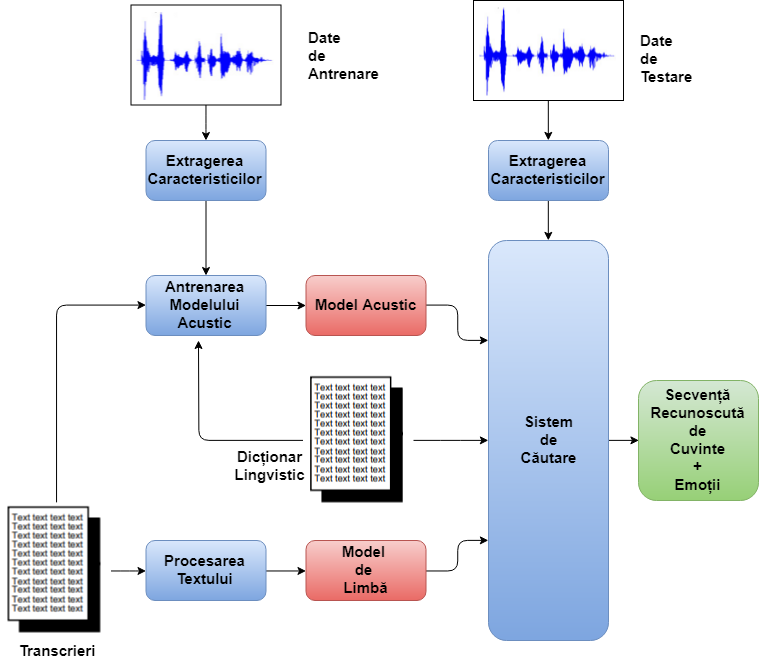
\includegraphics[width=\columnwidth]{res/fig/arhitectura-modelL-modelA}
\caption{Arhitectura unui sistem de recunoaștere a emoțiilor ce utilizează informația acustică și lingvistică}
\label{fig3}
\end{figure}

Modelul de limbă este realizat pe baza transcrierii cuvintelor, în paralel are loc extragerea de vectori de caracteristici din semnalul vocal. Vectorul rezultat împreună cu dicționarul de limbă sunt utilizate pentru a antrena modelele acustice de foneme. La recunoaștere sunt utilizate atât modelul acustic cât și cel de limbă pentru a putea recunoaște secvența după următoarea regulă:

\begin{equation} \label{eq1}
\begin{split}
\hat{W} & =arg \max_{{w}} P(W|Y) = arg \max_{{w}} \frac{P(W)P(Y|W)}{P(Y)} \\
 & =  arg \max_{{w}} P(W)P(Y|W)
\end{split}
\end{equation}

Formula utilizează funcția argmax, care selectează argumentul ce maximizează probabilitatea secvenței de cuvinte. Dezvoltarea din ecuația 1 are la bază regula Bayes și s-a făcut ținând cont de faptul că probabilitatea mesajului vorbit p(X) este independentă de secvența de cuvinte W. Ultimul rezultat evidențiază doi factori care pot fi estimați direct. Problema inițială (găsirea secvenței de cuvinte pe baza mesajului vorbit) a fost împărțită în două sub-probleme mai simple: a) estimarea probabilității apriori a secvenței de cuvinte p(W) și b) estimarea probabilității mesajului vorbit dată fiind secvența de cuvinte pronunțată p(X|W). Primul factor poate fi estimat utilizând exclusiv un model de limbă, iar cel de-al doilea poate fi estimat cu ajutorul unui model acustic. Cele două modele pot fi construite independent așa cum se va vedea în secțiunea următoare, dar vor fi folosite împreună pentru a decoda un mesaj vorbit, așa cum arată ecuația 1 \cite{b3}.

\subsubsection{Utilizarea informațiilor acustice, lingvistice și de discurs}
Indicatorii de discurs reprezintă expresii lingvistice care transmit informații explicite despre structura discursului sau au o contribuție semantică la aceasta. În contextul de recunoaștere a emoțiilor, informațiile legate de discurs mai prezintă și modul în care utilizatorul interacționează cu sistemul. Se întâmplă adesea ca utilizatorul să manifeste emoții in timpul interacțiunii cu sistemul, emoții cum ar fi frustrarea. Informațiile de discurs sunt combinate cu informațiile acustice pentru a îmbunătăți performanțele de recunoaștere.


\section{Metode de recunoaștere a emoțiilor}
În continuare se a prezenta o comparație între rezultatele obținute de două metode de recunoaștere a emoțiilor. Prima metodă se bazează pe utilizarea modele de mixturi Gaussiene antrenate pe baza caracteristicilor globale cum ar fi frecvența fundamentală și conturul energiei semnalului audio. A doua metodă utilizează modele Markov ascunse antrenate pe baza caracteristicilor locale ale semnalului audio. 

\subsection{Modele de mixturi Gaussiene}
Modelele de mixturi Gaussiene oferă o bună aproximare a caracteristicilor extrase din semnalul audio prin amestecul ponderat de densități Gaussiene. Coeficienții mixturilor s-au calculat cu ajutorul unui algoritm de maximizare a așteptării. Fiecare emoție este modelata într-un GMM. În experiment s-a remarcat un rezultat bun utilizând un număr de 16 mixturi Gaussiene.

\begin{figure}[htb]
\includegraphics[width=0.9\columnwidth]{res/fig/GMM}
\caption{Matricea de confuzie a analizei utilizând modele GMM \cite{b8}}
\label{fig4}
\end{figure}

 În tabel sunt următoarele abrevieri: sur - surprise, joy - joy, ang - anger, fea - fear, dis - disgust, sad - sadness și ntl - neutral \cite{b8}.



\subsection{Modele Markov ascunse}
Modelul HMM reprezintă un automat cu stări finite alcătuit dintr-un set de stări conectate între care se tranziționează. Secvența de stări a modelului HMM este ascunsă, cu toate
Matricea de confuzie a fost realizată utilizând 64 de stări și patru mixturi Gaussiene. 

\begin{figure}[htb]
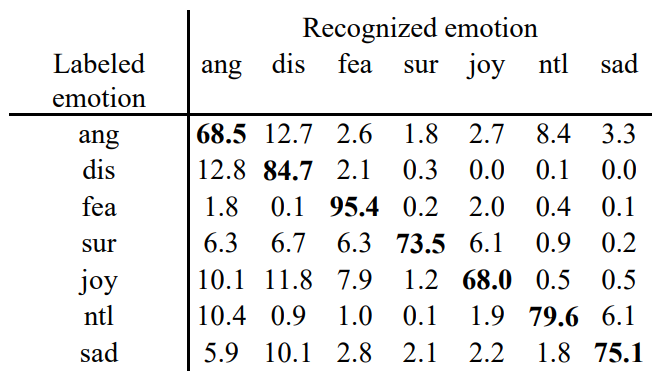
\includegraphics[width=0.9\columnwidth]{res/fig/HMM}
\caption{Matricea de confuzie a analizei utilizând modele HMM \cite{b8}}
\label{fig5}
\end{figure}

\section{Concluzii}
În acest document au fost prezentate câteva aplicații practice în care poate fi utilizat procesul de recunoaștere a emoțiilor pe baza semnalului vocal. De asemena au mai fost prezentate și principalele caracteristici pe baza cărora se face analiza semnalului și s-au prezentat rezultatele obținute în cazul utilizării a două metode distincte de recunoaștere a emoțiilor.Ambele metode prezentate s-au dovedit a fi capabile să identifice emoțiile din mesaje audio vocale. Tabelele de confuzie arată clar că unele emoții sunt confundate între ele, ceea ce indică similitudini între caracteristicile emoțiilor. De asemenea, aceste rezultate din tabelul de confuzie mai pot fi influențate și de faptul că datele utilizate la antrenare nu au avut cea mai bună calitate din punctul de vedere al calității emoțiilor. Din cele două tabele se remarcă faptul că utilizarea caracteristicilor globale oferă rezultate mai bune decât utilizarea caracteristicilor locale. 

\begin{thebibliography}{00}

\bibitem{b1} Moataz El Ayadi, Mohamed S. Kamel, Fakhri Karray : ``Survey on speech emotion recognition: Features, classification schemes, and databases''

\bibitem{b2} validare în vruce: https://www.openml.org/a/estimation-procedures/1

\bibitem{b3} Horia Cucu: ``Proiect de cercetare-dezvoltare în Tehnologia Vorbirii''

\bibitem{b4} Senaka Amarakeerthi, Rasika Ranaweera, and Michael Cohen: Speech-based Emotion Characterization using Postures and Gestures in CVEs

\bibitem{b5} Vicki R. LeBlanc • Meghan M. McConnell • Sandra D. Monteiro: ``Predictable chaos: a review of the effects of emotions on attention, memory and decision making''

\bibitem{b6} Paul Ekman: ``Emotions Revealed''

\bibitem{b7} Jonghwa Kim, Elisabeth Andre: ``Emotion Recognition Based on Physiological Changes in Music Listening''

\bibitem{b8} Björn Schuller, Gerhard Rigoll, and Manfred Lang: ``HIDDEN MARKOV MODEL-BASED SPEECH EMOTION RECOGNITION''

\end{thebibliography}
\end{document}
